% !TeX root = ../../../master.tex

\subsection{Aufbau React}
\label{ssec:AufbauReact}

Um React bzw. den Komponentenaufbau zu verstehen, muss man sich darüber im klaren sein, was die Komponenten können. 
Hierzu zählt u.a. das Verständis, dass eine Komponente Parameter übermittelt bekommen kann (\props). 
Wie auch in anderen Programmiersprachen wie z.B. Java, wird bei den Komponenten ein Konstruktor \engl{constructor} verwendet.
Dieser erlaubt es Zugriff auf die übermittelten \props. 

Die Hauptmethode einer Komponente ist die \render-Funktion. 
Sie definiert das Aussehen der Komponente, welches deskriptiv über \acs{HTML} oder weitere Kind-Komponente(n) beschrieben wird. 
Wichtig zu verstehen ist hierbei, dass beim Laden einer solchen Komponente mind. zwei interne Funktionen aufgerufen werden. 
Zum einen wird beim Laden die Funktion \cwm aufgerufen, die Änderungen vor dem kompletten Laden der Komponente vollzieht. Dies sollte jedoch ab der Version 17 nicht mehr verwendet werden. 
Zum zweiten wird nach dem Erstellen der Komponente die Funktion \cdm aufgerufen. 
Diese ermöglicht es z.B. den \state  der Anwendung zu verändern. 
Ein Beispiel hierfür wäre das Formularfeld, welches als \props den Vor-, Nachname und Alter eines Studentes erhält. 
Diese Änderungen erfolgt lediglich auf der zu änderten Komponente über den virtuellen \acs{DOM}. 
Das Ändern des \state wird über eine Funktion \exampleState durchgeführt, welches die neuen Parameter in der Komponente setzt. \todo[]{Niko: Name und value muss in Klammer}
Dadurch, dass React nur die Teile bzw. Komponenten ändert, an den Änderungen aufgetreten sind, erhält man zudem eine erhöhte Performance im Bezug auf Ladegeschwindigkeit, da nicht die komplette Seite neu gerendert wird. 

\begin{figure}[!h]
	\centering
	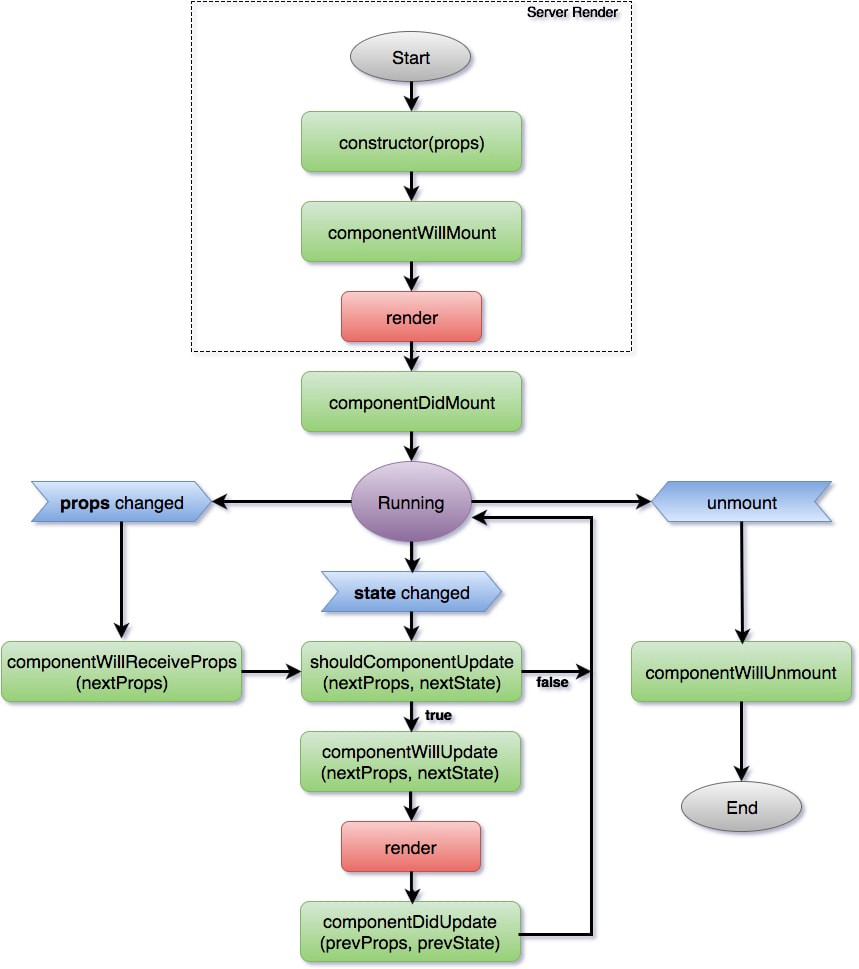
\includegraphics[width=0.70\textwidth, keepaspectratio]{img/client/Lifecycle.jpeg}
	\captionsetup{justification=centering, format=plain}
	\caption[Aufbau React]{Aufbau React \\ \quelle \cite{reactLifeCycle}}
	\label{fig:ReactLifecylce}
\end{figure}
